% !TeX spellcheck = pt_PT
\documentclass[a4paper]{report}
\usepackage[portuguese]{babel}
\usepackage{a4wide}
\usepackage[utf8x]{inputenc}
\usepackage[utf8]{inputenc}

\usepackage{graphicx}
\usepackage{hyperref}
\usepackage{listings}
\usepackage{indentfirst}
\usepackage{float}
\usepackage{color}

\setlength{\parskip}{1em}

\definecolor{mygreen}{rgb}{0,0.6,0}
\definecolor{mygray}{rgb}{0.5,0.5,0.5}
\definecolor{mymauve}{rgb}{0.58,0,0.82}

\lstset{ %
  backgroundcolor=\color{white},   % choose the background color
  basicstyle=\footnotesize,        % size of fonts used for the code
  breaklines=true,                 % automatic line breaking only at whitespace
  captionpos=b,                    % sets the caption-position to bottom
  commentstyle=\color{mygreen},    % comment style
  escapeinside={\%*}{*)},          % if you want to add LaTeX within your code
  keywordstyle=\color{blue},       % keyword style
  stringstyle=\color{mymauve},     % string literal style
}

\title{POO - Trabalho Prático\\
	\large Grupo nº13}

\author{Ivo Miguel Gomes Lima \\ (A90214) \and Miguel Ângelo Alves de Freitas \\ (A91635)
         \and Tiago dos Santos Silva Peixoto Carriço \\ (A91695)
       } %autores do documento
       
\date{\today} %data

\begin{document}
	\begin{minipage}{0.9\linewidth}
        \centering
		
\includegraphics[width=0.4\textwidth]{um.jpg}\par\vspace{1cm}
		\href{https://www.uminho.pt/PT}
		{\scshape\LARGE Universidade do Minho} \par
		\vspace{0.6cm}
		\href{https://lcc.di.uminho.pt}
		{\scshape\Large Licenciatura em Ciências da Computação} \par
		\maketitle
		\begin{figure}[H]
			
\includegraphics[width=0.32\linewidth]{ivo.jpg}
			
\includegraphics[width=0.32\linewidth]{miguel.jpg}
			
\includegraphics[width=0.32\linewidth]{tiago.jpg}
		\end{figure}
	\end{minipage}
	
	\tableofcontents
	
	\pagebreak
	
	\chapter{Introdução e principais desafios}
%	
	Este projeto consistiu no desenvolvimento de uma aplicação semelhante ao Football Manager na linguagem de programação Java, de forma a pôr em prática os conhecimentos adquiridos ao longo do semestre. 
	
	Consideramos que o maior desafio seja o impedimento da comunicação entre a simulação de jogo e a \emph{view}.
	
	\chapter{Classes}
	
	\section{Jogador}
	\begin{lstlisting}[language=java]
    private String nome; // Nome do jogador
    private String equipa; // Nome da equipa
    private int id; // Identificador do jogador (valor unico)
    private ArrayList<String> historico; // Historico de equipas
    private Map<String,Integer> atributos; // Atributos do jogador
	\end{lstlisting}
	
	Começamos por fazer uma classe mais geral, onde temos os identificadores gerais representados a cima. Com isto podemos proceder à criação de um jogador mais genérico onde identificamos os jogadores, os seus atributos, nomes, equipas a que pertence, número da camisola e o seu histórico.
	
	\section{Guarda-Redes}
	\begin{lstlisting}[language=Java]
    private int elasticidade;
	\end{lstlisting}
	
	\textbf{"Guarda-Redes"} é uma classe mais específica da classe "Jogador", ou seja, é uma subclasse onde vamos atribuir peso específico como o acima assinalado, pois no nosso ponto de vista é uma especialização importante dos Guarda-Redes num jogo de futebol.
	
	\section{Lateral}
	\begin{lstlisting}[language=Java]
    private int cruzamento;
    private int drible;
	\end{lstlisting}
	
	\textbf{"Lateral"} é uma classe mais específica da classe "Jogador", ou seja, é uma subclasse onde vamos atribuir pesos específicos como os acima assinalados, pois no nosso ponto de vista são as especializações dos laterais num jogo de futebol.
	
	\newpage
	
	\section{Defesa}
	\begin{lstlisting}[language=Java]
    private int corte;
    private int intersecao;
	\end{lstlisting}
	
	\textbf{"Defesa"} é uma classe mais específica da classe "Jogador", ou seja, é uma subclasse onde vamos atribuir pesos específicos como os acima assinalados, pois no nosso ponto de vista são as especializações dos defesas num jogo de futebol.
	



	\section{Médio}
	\begin{lstlisting}[language=Java]
    private int intersecao;
    private int visao;
	\end{lstlisting}
	
	\textbf{"Médio"} é uma classe mais específica da classe "Jogador", ou seja, é uma subclasse onde vamos atribuir pesos específicos como os acima assinalados, pois no nosso ponto de vista são as especializações mais imporantes dos médios num jogo de futebol.
	
	\section{Avançado}
	\begin{lstlisting}[language=Java]
    private int finalizacao;
    private int compostura;
	\end{lstlisting}
	
	\textbf{"Avançado"} é uma classe mais específica da classe "Jogador", ou seja, é uma subclasse onde vamos atribuir pesos especificos como os acima assinalados, pois no nosso ponto de vista são as especializações dos avançados num jogo de futebol.
	
    \section{Equipa}
	\begin{lstlisting}[language=Java]
    private String nome;
    private Map<Integer,Jogador> jogadores;
    private int[] titulares;
	\end{lstlisting}
	
    \textbf{"Equipa"} é uma classe abrangente onde vamos adicionar os jogadores, removê-los, definir se o jogador é titular, calcular o overall da equipa e/ou dos jogadores titulares. Também nesta classe temos métodos para conseguirmos obter a equipa completa e mudar conforme as devidas substituições em jogo. Podemos modular as equipas fazendo tranferências de jogadores e possibilitando ainda a chamada da classe \emph{parse} para a leitura do ficheiro.
	
	
    	\newpage
    	
    	
	\section{Jogo}
	\begin{lstlisting}[language=Java]
    private String equipaCasa;
    private String equipaFora;
    private int golosCasa;
    private int golosFora;
    private LocalDate date;
    private List<Integer> jogadoresCasa;
    private List<Integer> jogadoresFora;
    private Map<Integer, Integer> substituicoesCasa; // sai -> entra
    private Map<Integer, Integer> substituicoesFora; // sai -> entra
	\end{lstlisting}
	
	Nesta classe são guardados todas as informações de um jogo, nomeadamente os nomes dos jogadores, nomes das equipas, número de golos, a data do evento, jogadores titulares assim como as substituições feitas.
	
    
    
	\section{Parser}
	\begin{lstlisting}[language=Java]
	\end{lstlisting}
	\emph{"Parser"} é uma classe feita pela equipa de docente da disciplina, mas tendo algumas alterações da nossa parte para adaptar ao nosso código. Esta classe vai permitir ler todo o texto de um ficheiro, organizando as equipas, as posições e os jogos já realizados.
	

	
	\section{SaveGame}
	\begin{lstlisting}[language=Java]
	\end{lstlisting}
	
	\emph{"SaveGame"} é uma classe onde enviamos todas as informações relevantes dos jogos para serem guardadas, ou seja, vamos guardar o estado atual das equipas, e todos realizados para que possam ser posteriormente guardados num ficheiro .txt que será interpretado pela classe \emph{parser}.
    
     	\newpage
     	
	\section{SimulacaoJogo}
	\begin{lstlisting}[language=Java]
    private static final int CASA = -1;
    private static final int MEIO = 0;
    private static final int FORA = 1;

    private Jogo jogo;
    private Equipa equipaCasa;
    private Equipa equipaFora;
    private int overallCasa;
    private int overallFora;
    private int posseBola;
    private final int posseIntervalo;
    private int posicaoBola;
    private int substituicoesCasa;
    private int substituicoesFora;
	\end{lstlisting}
	
	Esta classe vai representar a simulação de um jogo de futebol real entre duas equipas, a de casa e a de fora, necessitando das informações dos constituintes de ambas as equipas assim como os seus \emph{overalls}. O algoritmo que utilizamos para esta simulação baseia-se em:
	\begin{itemize}
        \item O campo está divido em 3 partes(área da equipa de casa, meio campo, área da equipa de fora).
        \item Em cada jogada, a equipa atacante pode suceder e avançar para o terço seguinte, se estiver no último terço marca golo, em caso de insucesso a posse de bola muda para a equipa adversária e dá-se um contra-ataque.
        \item Ao longo das jogadas, pode dar-se um momento de substituição, onde o utilizador fará a escolha.
    \end{itemize}
	 Este algoritmo é efetuado duas vezes, pois existe divisão de partes.
	
\newpage
	
	\section{View}
	\begin{lstlisting}[language=Java]
    private Controller controller;
    private Scanner input;
	\end{lstlisting}
	
	A \emph{view} é a Vista do programa. Comunica apenas com o Controller. Possui vários métodos, pricipalmente métodos para mostrar algum tipo de informação ao utilizador ou mensagens de erro. Mantendo a identididade da arquitetura (Model-View-Controller).
    
    \section{{\large Menu}}
    O jogo FM incializa com este menu e uma mensagem de texto. Possui as seguintes opções:
	
                    \textit{"0.Sair"} - Sair do Jogo FM
                    
                    \textit{"1.Carregar ficheiro"} - Carrega uma lista de equipas e jogos através um ficheiro .txt, seguindo a estrutura é a indicada pela equipa docente
                    
                    \textit{"2.Gravar estado em ficheiro"} - Grava o estado atual do jogo e tudo que nele se encontra num ficheiro .txt.
                    
                    \textit{"3.Carregar ficheiro de objetos"} - Faz o mesmo que o anterior mas carrega em ficheiro objeto em vez de .txt.
                    
                    \textit{"4.Gravar estado em ficheiro de objetos"} - Faz o mesmo que o anterior mas grava em ficheiro objeto em vez de .txt.
                    
                    \textit{"5.Criar Equipa" } - Permite ao utilizador criar uma nova equipa vazia para que possam ser adicionados jogadores.
                    
                    \textit{"6.Adicionar Jogador" } - Permite ao utilizador criar um jogador onde e adicionar a uma equipa à sua escolha. Caso não existam equipas só é possível adicionar à equipa "jogadores sem equipa".
                    
                    \textit{"7.Transferir Jogador"} - Permite ao utilizador transferir qualquer jogador entre equipas guardando no histórico do jogador essa transferência.
                    
                    \textit{"8.Remover Equipa"} - Permite ao utilizador remover uma equipa e, por defeito, todos esses jogadores são atribuidos à equipa "jogadores sem equipa".
                    
                    \textit{"9.Remover Jogador"} - Permite ao utilizador remover definitivamente um jogador de qualquer equipa.
                    
                    \textit{"10.Simular Jogo"} - Permite a realização de um jogo entre duas equipas definidas pelo utilizador.
                    
                    \textit{"11.Informação"} - Nesta opção podemos encontrar todas as informações extra-Jogo, ou seja, consultar mais dados referente à equipa e informações referentes aos jogadores.
                    
                    
	\newpage
	
	\section{Controller}
	\begin{lstlisting}[language=Java]
    private static final int CASA = -1;
    private static final int FORA = 1;
    private Map<String,Equipa> equipas;
    private List<Jogo> jogos;
    private SimulacaoJogo simulacao;
	\end{lstlisting}
	
	Esta classe, juntamente com outras, direciona o fluxo da aplicação mapeando e direcionado as ações recebida (request) pela camada da apresentação para os respectivos serviços da aplicação. Esta classe vai ser responsável pela gestão do menu inicial, além de interagir com outras classes controladores que gerem os menus da view, fazendo todo o trabalho "lógico" da view.	
	
	\section{Interface}
	\begin{lstlisting}[language=Java]
	\end{lstlisting}
	
	Esta classe é a classe principal que inicializa as componentes necessárias para o funcionamento do Modelo MVC.
	
	
	
	
	\chapter{Exceptions}
	
    \section{EquipaNaoDefinidaException}
	
    Esta exception foi criada no âmbito de quando a equipa não é definida ou quando é definida incorretamente, alertando o utilizador para este problema.
    
    \section{EquipaJaExisteException}
	
    Esta exception foi criada no âmbito de quando a equipa já está definida e impede a sobreposição de comandos sobre a mesma, alertando o utilizador para este problema.
	
	\section{NumeroInvalidoException}
	
	Esta exception foi criada no âmbito de quando um dos jogadores não é definido ou quando é definido incorretamente, alertando o utilizador para este problema.
	
	\section{JogadorNaoExisteException}
	
	Esta exception foi criada no âmbito de quando um dos jogadores não está definido ou foi definido de forma incorretamente, alertando o utilizador para este problema.
	
	
	\section{JogadorJaExisteException}
	
	Esta exception foi criada no âmbito de quando um dos jogadores é definido e já existe na equipa, alertando o utilizador para este problema.
	
	\section{LinhaIncorretaException}
	
	Esta exception foi criada no âmbito de quando uma das linhas está de forma incorreta, alertando o utilizador para este problema.  
	
	\section{SubstituicaoErradaException}
	
	Esta exception foi criada no âmbito de quando na fase do jogo a substituição não é feita corretamente, alertando o utilizador para este problema.
	
	\section{TitularesNaoDefinidosException}
	
	Esta exception foi criada no âmbito de quando os titulares não foram definidos corretamente, na inicialização do jogo ou durante, alertando o utilizador para este problema.
	
	\section{SimulaçãoImpossivelException}
	
	Esta exception foi criada no âmbito de caso exista algum erro numa definição ou alguma atribuição do utilizador a simulação não se realizar, alertando o utilizador para este problema.
	
	
	

	\chapter{Estrutura do projeto}

	O nosso projeto segue a estrutura \textit{Model View Controller} (MVC), estando por isso organizado em três camadas:
	\begin{itemize}
		\item A camada de dados (o modelo) é composta pelas Classes Jogador, Guarda-Redes, Lateral, Defesa, Médio, Avançado, Equipa, Jogo e Simulacao pelas interfaces.
		\item A camada de interação com o utilizador (a vista, ou apresentação) é composta unicamente pela classe View.
		\item A camada de controlo do fluxo do programa (o controlador) é composta pela classe Controller.
	\end{itemize}
      Como foi referido anteriormente, todo o projeto baseia-se na ideia de encapsulamento.
      

      

	
	\chapter{Diagrama de Classes}
	\begin{figure}[H]
		\begin{center}
			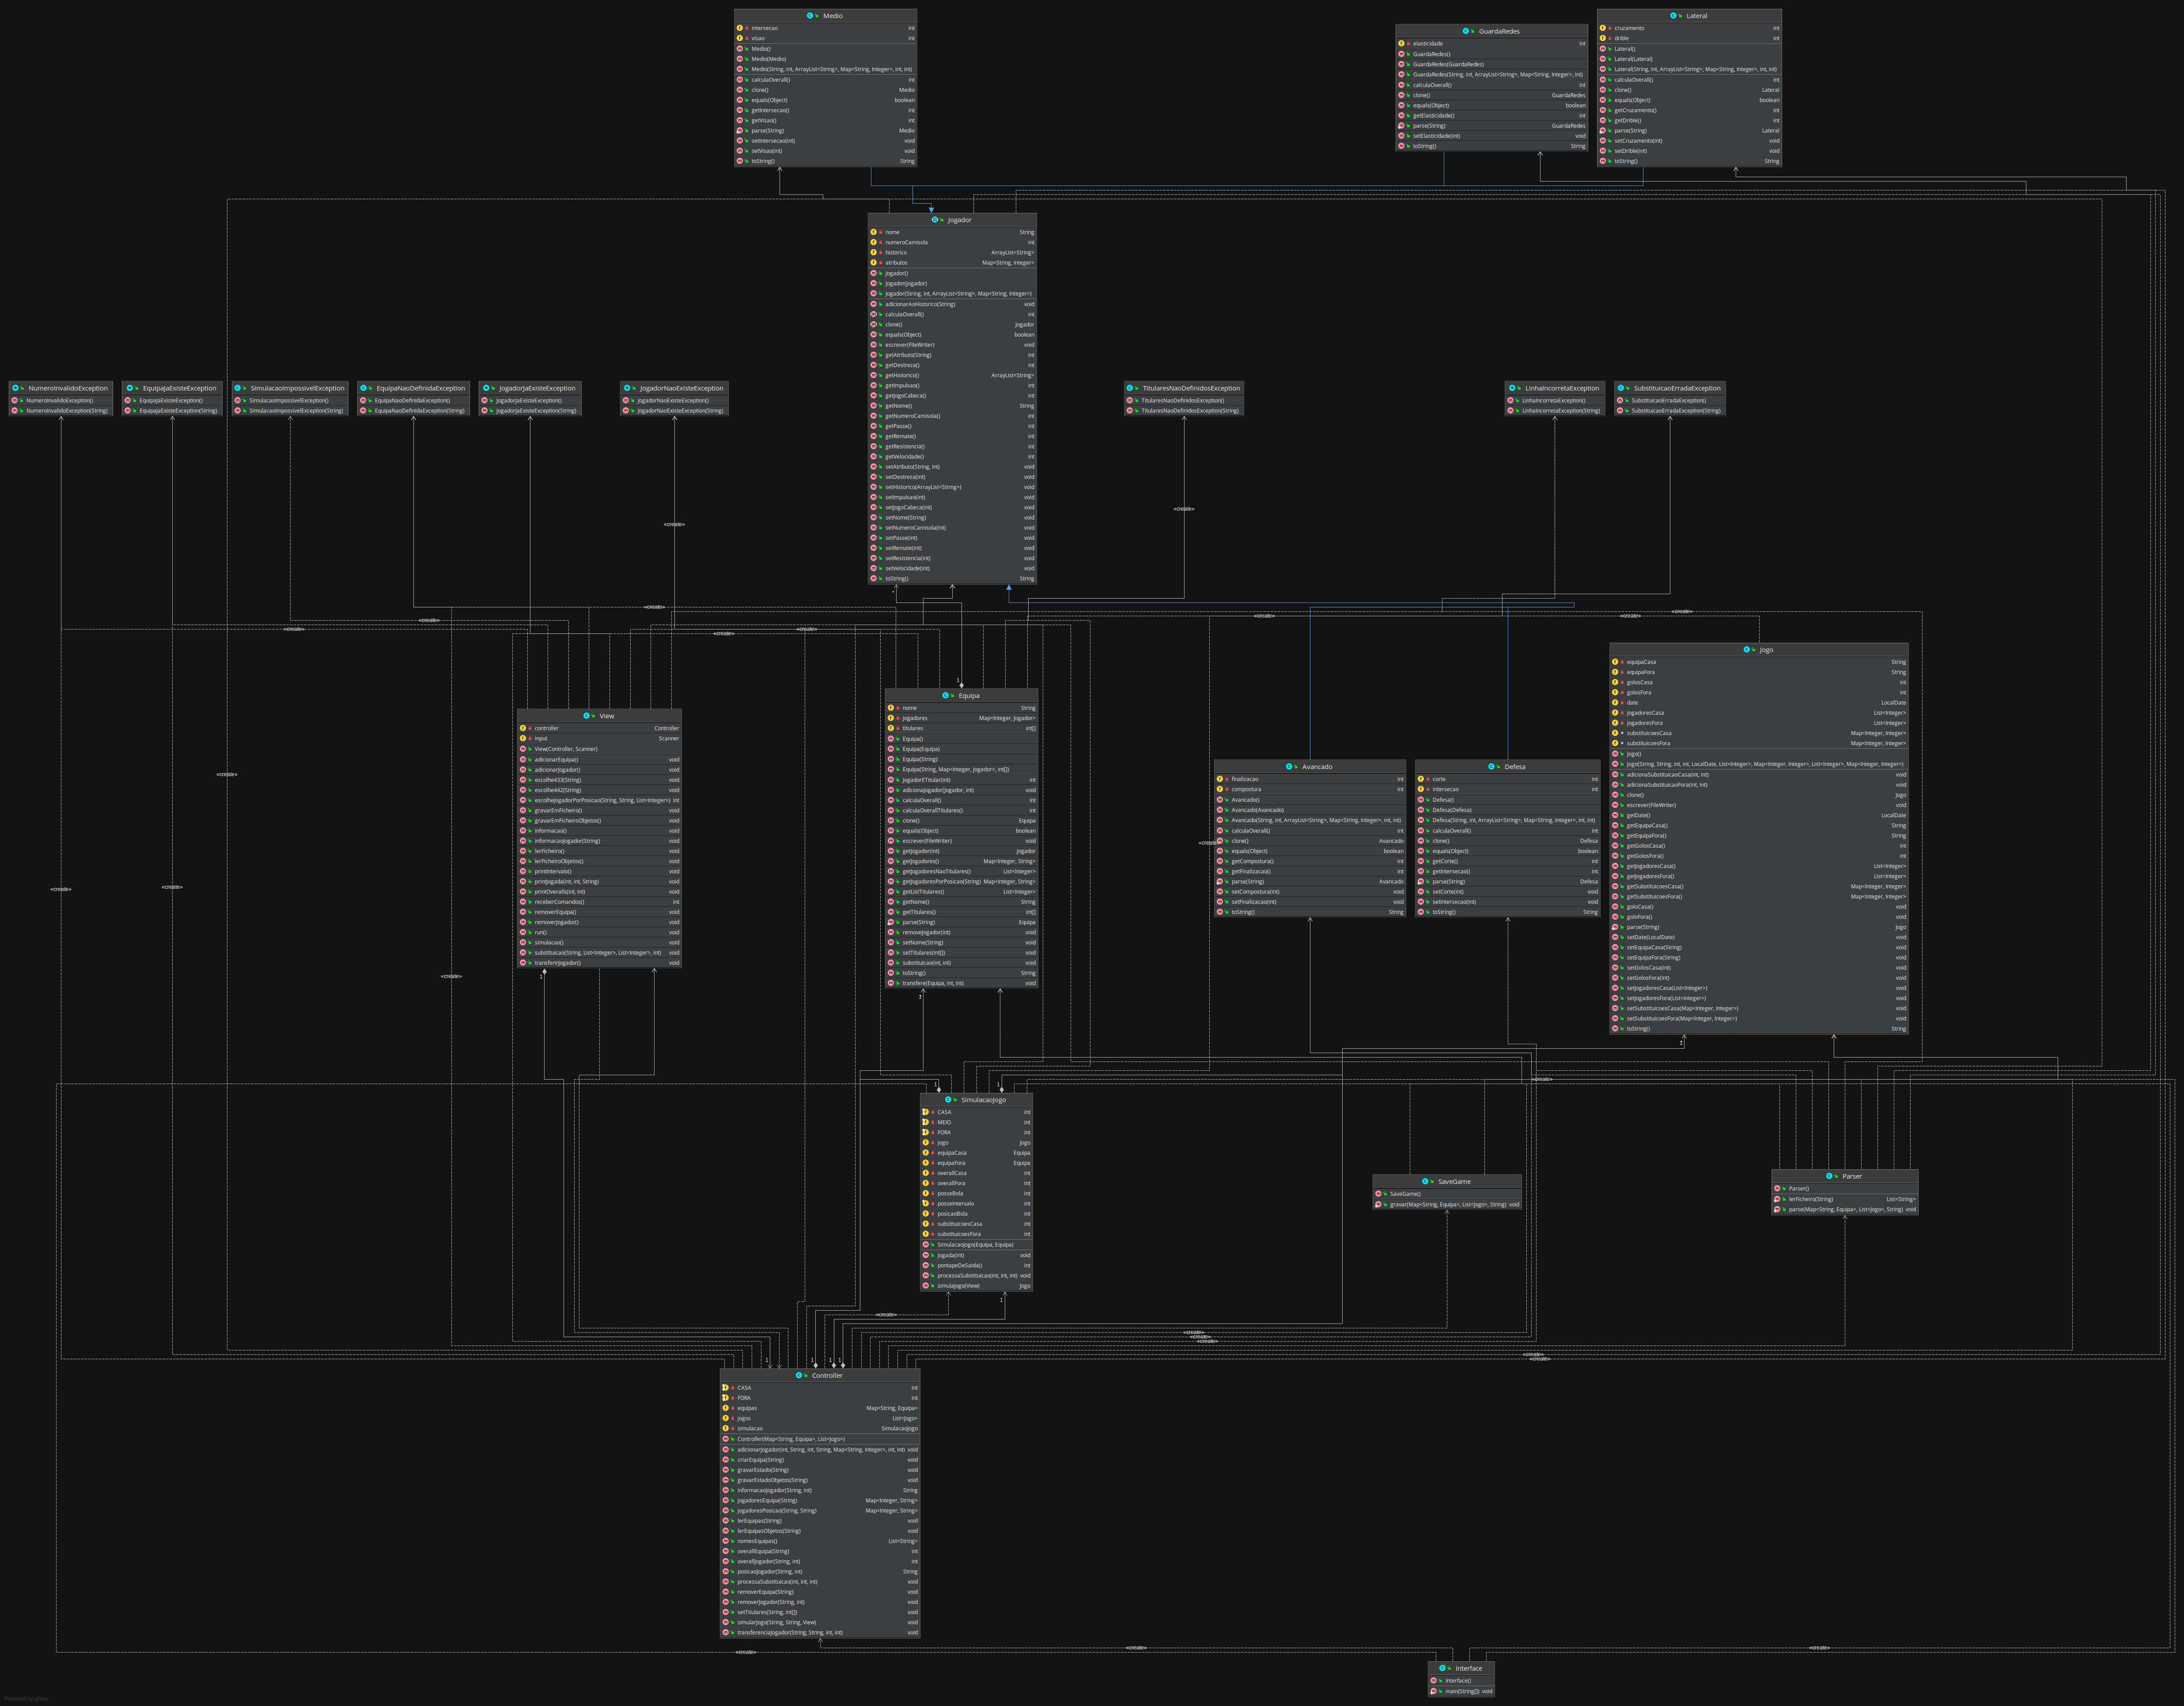
\includegraphics[height=0.6\textheight]{diagramaSemTeste.jpg}
			\caption{Diagrama de classes do programa, gerado pelo \emph{IntelliJ}}
		\end{center}
	\end{figure}	

	\chapter{Conclusão}

	A nível geral, e tendo em conta o que foi explicado nos capítulos anteriores, como grupo achamos que todos os objetivos foram cumpridos e apesar das dificuldades que fomos encontrando o grupo conseguiu superar de uma forma muito boa, sempre com um olhar crítico e a pensar no próximo passo. Acreditamos que respondemos de forma correta ao problema apresentado pela equipa docente da disciplina.
	
	

\end{document}
